\section{ General Framework for Group Deviation Detection
}
 \label{Sec:Framework}
In the last section, we clearly defined the problem of detecting group deviations in static and dynamic situations.   
  This section elaborates  upon the general framework and underlying structure for GAD and GCD techniques. Discovering significant group deviations is related to three sub-problems. 
\begin{enumerate}[1.]
\item {\it Group Structures}:  The definition of groups and the relationship between data instances is important to understand. %  clustering algorithm aggregate data instances into group structures.
\item {\it Statistical Properties}:  
A variety of statistical properties may characterise group deviations. % For example, a user is able to examine statistical properties of interest such as proportions, location or dependence.
 If statistical properties  are  not adequately quantified then relevant group deviations cannot be identified.
\item  {\it Model Design}: 
 The design of GAD and GCD techniques include data inputs,   model assumptions, learning approaches and output information. 
\end{enumerate}


\subsection{Group Structures}
We now highlight examples of different problems associated with group structures.   A group is a collection of two or more related data instances where Tan et al.  \cite{Tan} state that a data instance is synonymous with terms such as  vector, sample, entity, observation, etc. %Many GAD techniques assume that features from members in a group are independent and identically distributed (iid) where
Members in a group can be related by  external information of known group labels such as in topic modelling where Xiong et al. \cite{FGM} consider a document as a group of  words or a corpus as a group of documents. When group structures are not previously known, clustering algorithm aggregate data instances based on similarity criterion. 
 For example, Xiong et al. \cite{MGM} infer a spatial cluster of galaxies with distances closer than 1 megaparsecs while Wong et al. \cite{wong-rule} examine a demographic group of patients  based on certain categorical features.  
%   The interpretation of results relies on initial definition and construction of group structures. 
  
When group structures are unknown a priori,  clustering algorithms are applied. Common procedures minimise the cumulative  distance  between  members in a group to a central reference point. %These algorithms such as $k$-means or  nearest neighbors
 Clustering algorithm  for numerical values  are discussed in Jain \cite{jain2010} where a group of data instances contains members with similar features based on minimising distance metrics.   
Steinbach \cite{steinbach2004} discusses issues with distance-based clustering algorithms as data points become difficult to differentiate in higher dimensions.   More sophisticated techniques have been specifically developed for group  
%In particular,
 group deviation detection   %techniques infer clusters based on different criterion 
 such as:
\begin{enumerate}[-]
\item Chen et al.  \cite{GLETS}  apply density-based spatial clustering based on Pearson's correlation and Euclidean distance between values of times series. 
%\item Chen et al.  \cite{Chen2014} examine Pearson's correlation and Euclidean distance between values of times series.  
\item    Yu et al. \cite{GLAD} examine individual features as well as pairwise connection data.  %infer groups containing a mixture of social roles for social media applications. 
\item Soleimani and   Miller \cite{ATD} infer anomalous clusters of documents based on likelihood probabilities.
\item Dai et al. \cite{ERACD} cluster based on the ranking of feature values. 
\end{enumerate}
Therefore there are many procedures for clustering data instances when group structures are previously unknown.


\begin{figure}[h]
\centering
   \begin{subfigure}{1\linewidth} \centering
     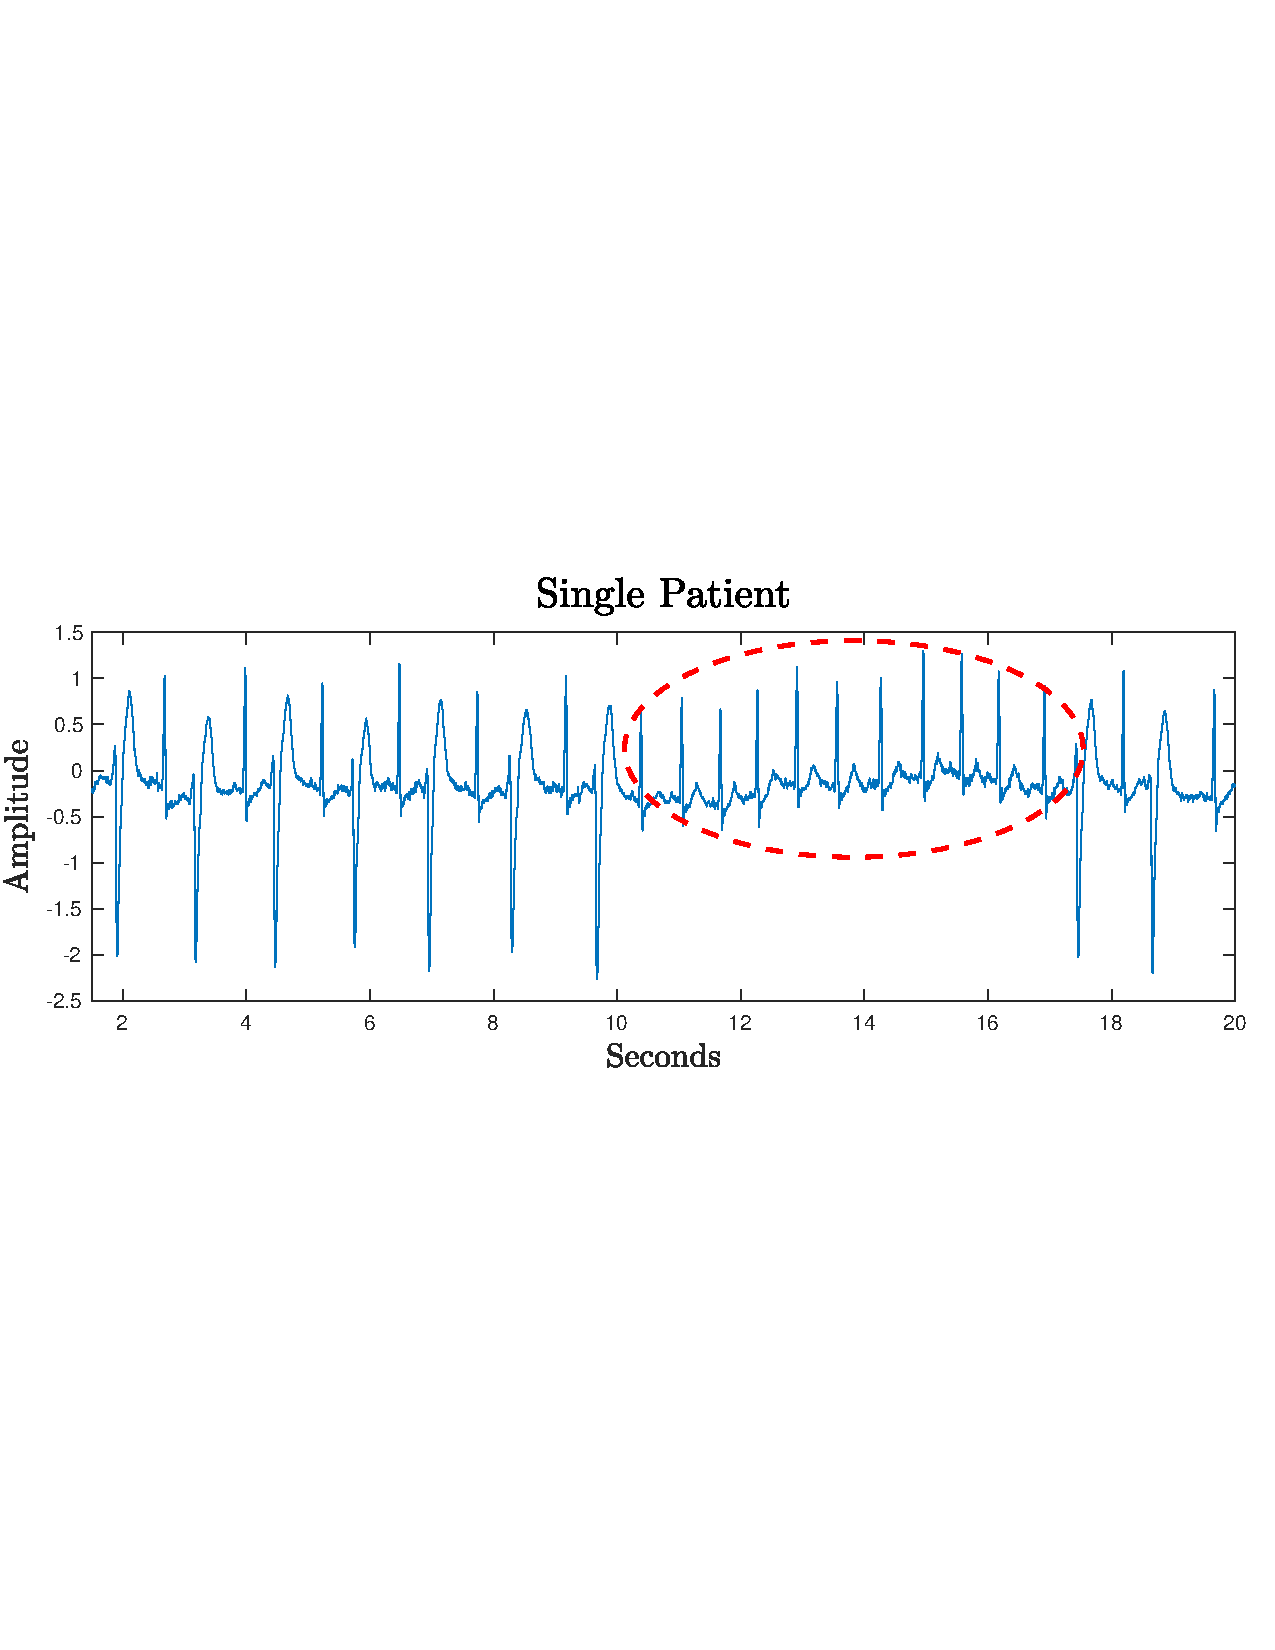
\includegraphics[width=6cm, height=4cm,trim=5cm 9.5cm 4.5cm 9cm]{FIGURES/ECGa}
     \caption{A collective anomaly (red dotted circle) in the ECG reading of a single patient.}
   \end{subfigure}
   \begin{subfigure}{1\linewidth} \centering
     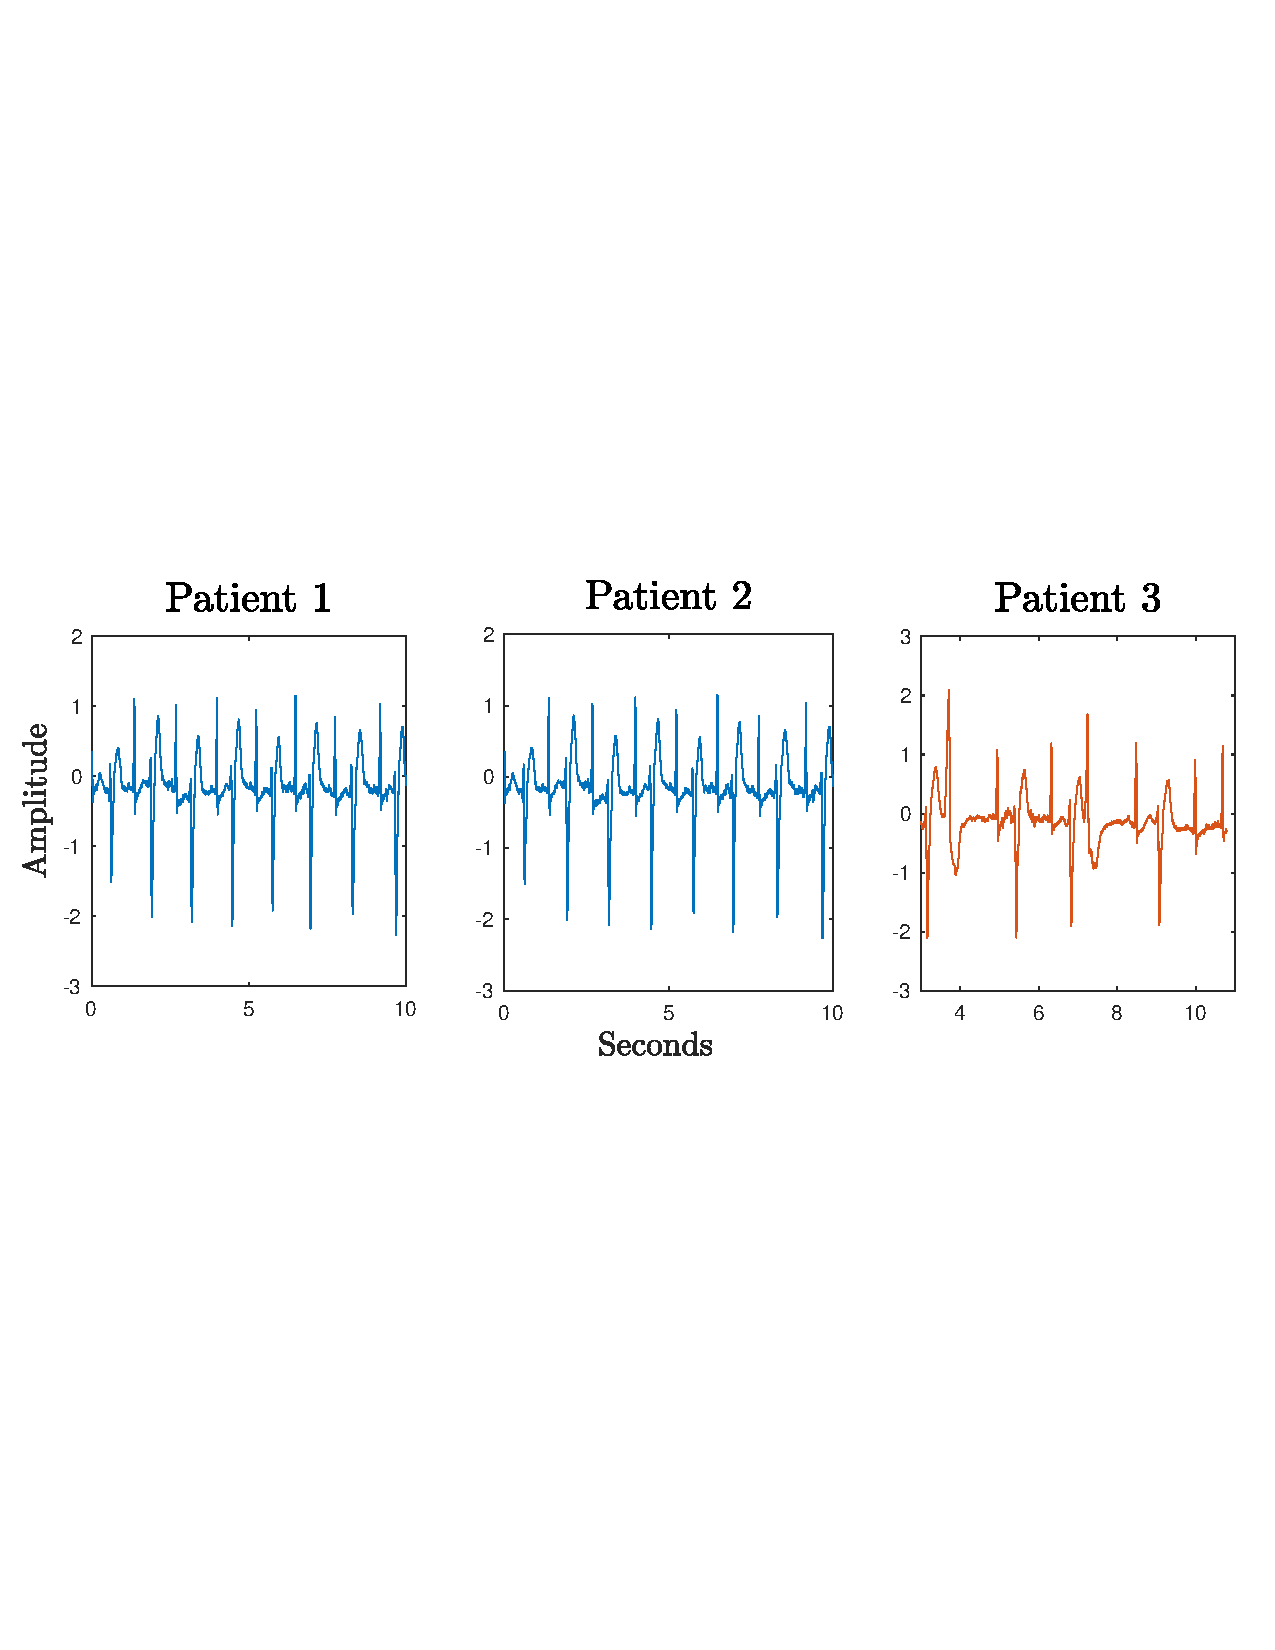
\includegraphics[width=6cm,  height=4cm,trim=5cm 9.5cm 4.5cm 8.5cm]{FIGURES/ECG}
     \caption{A group anomaly (Patient 3) is observed when comparing several patients.} 
   \end{subfigure}
  % \vspace{-1cm}
\caption{ In (a), a collective anomaly is a collection of related data instances that is anomalous with respect to time-dependent observations from  a single patient.   
In (b), a group anomaly is a specific example of a collective anomaly where  the entire dataset involves a group of observations from multiple patients. 
 } \label{Fig:ECG}
\end{figure}
%\vspace{1cm}


 
 
In our thesis, we do not use group anomaly and  collective anomaly interchangeably.  Chandola \cite{Chandola} defines a collective anomaly  as "a collection of related data instances that is anomalous with respect to the entire dataset." 
A group anomaly is specific example of a collective anomaly where  
the entire dataset involves multiple groups. % in the dataset. 
To differentiate these terms, consider the electrocardiogram (ECG) example from Goldberger et al. \cite{Goldberger}.  Figure \ref{Fig:ECG} (a) highlights a collective anomaly (in the dotted red circle) that exhibits an irregular pattern as compared to the  entire dataset (time series of a single patient). For a GAD application,  Figure \ref{Fig:ECG} (b) illustrates ECG readings from several patients  where  Patient 3 represents a group anomaly as the statistical properties are significantly different.  %however this is also a collective anomaly as the entire dataset can be considered as information from all of the patients.
 A realistic GCD case  would involve a group of patients with ECG readings similar to Figure \ref{Fig:ECG} (a) where a large-scale phenomena affects all patients around $\tau=10$. 
 


\subsection{Statistical Properties}
% SP - known vs unknown
 In some cases, a domain expert is interested in particular  statistical properties of groups. Statistical properties are measured and compared for group deviation detection. In terms of point-based and distributed-based group behaviours, point-based group deviations are characterised by a central location while distributed-based group deviations are characterised by statistical properties other than location such as scale, shape or dependence. In practice, group deviations are difficult to detect as a combination of statistical properties may  significantly differ. If a user is able to specify statistical properties of interest, group deviations are more easily detected and interpreted. 

 Since there are also many ways to quantify statistical properties of groups, we describe common parametric and non-parametric measures for statistical properties in Table \ref{Tab:Des} where non-parametric measurements are more robust to individual outliers. %Statistical properties in Table \ref{Tab:Des}, capture group  behaviours  for continuous variables however other metrics are more suitable for discrete or categorical datasets. 
   Given prior knowledge of statistical properties that characterise group deviations for GAD or GCD applications, a suitable method for discriminating groups is easily constructed. However when the nature of significant group deviations in terms of statistical properties is unknown, more   specialised techniques are required.  
 
 
		\begin{table}[h]
%\renewcommand{\arraystretch}{1}
	\tabcolsep=0.1cm
	\begin{center}
   \scalebox{0.88}{
	\begin{tabular}{lccc  }
	\hline\\[-2mm]
		%\multirow{ 2}{*}{} & & & \\[2mm]
 Statistical & %Function &
	 Parametric Measures% in $\boldsymbol \alpha$ 
	 &  Non-parametric Measures %  in  $\boldsymbol \gamma$ 
	 \\[-1mm]  Property & & &
	 \\[2mm] \hline\\[-2mm]
		\multirow{ 2}{*}{Location } & %	\multirow{ 2}{*}{$h_1$ }&
	  $ \displaystyle\bar{ {X}}_v=\frac{1}{N} \sum_{n=1}^N X_{nv}$ & $  \displaystyle \hat{q}_v({0.5})$  \\
	 & \hspace{5mm}(mean) & (median)  \\%[2mm]
	  %
	\multirow{ 2}{*}{Scale} & %\multirow{ 2}{*}{$h_2$} &
	 $ \hat\sigma^2_v = \displaystyle	\frac{1}{N-1}\sum_{n=1}^{N} \big(X_{nv}-\bar {X}_v \big)^2$  &  % \displaystyle s^2 =	\(\stackunder[1pt]{$ \mbox{mediai}$}{	\scalebox{0.8}{$ 1\le i\le N$}} \) $\big (| X_n - q_{0.5}| \big)$ 
	$\displaystyle \hat{q}_v({0.75}) - \hat{q}_v({0.25})$ \\ %[-1mm]
	 & (variance) &(interquartile range)   \\[1mm]
	 Skewness & % $h_3$ &
	$\displaystyle\frac{1}{N} \sum_{n=1}^N \frac{( X_{nv}-\bar{X}_v)^3}{ \hat\sigma_v^3}  $  & 
	$ \displaystyle \frac{\hat{q}_v({0.9}) + \hat{q}_v({0.1}) -2 \hat{q}_v({0.5}) }{  \hat{q}_v({0.9}) - \hat{q}_v({0.1})  }$\\[4mm] %\displaystyle  \hat{\mathcal{S}}=
	 Kurtosis &  %$h_4$ &
	 $\displaystyle\frac{1}{N} \sum_{n=1}^N \frac{( X_{nv}-\bar{X}_v)^4}{ \hat\sigma_v^4}  $ &
	$ \displaystyle\frac{\hat{q}_v({0.975}) -\hat{q}_v({0.025}) }{\hat{q}_v({0.75}) -\hat{q}_v({0.25}) }  $ \\[4mm] %\displaystyle \hat{\kappa} =
	 	\multirow{ 2}{*}{Dependence} &  	%\multirow{ 2}{*}{$H$} &
	  $ \; %\hat \rho =
	   \displaystyle\frac{ \sum_{n} \big(X_{n1}- \bar X_{1} \big) \big(X_{n2} - \bar X_{2}\big) } {\sqrt{ \sum_n \big(X_{n1}- \bar X_{1} \big) ^2 \sum_n \big(X_{n2} - \bar X_{2}\big)^2 }   } $ & 
	\;\; $\displaystyle   \frac{ \sum_{n} \big(R_{n1} - \bar R_{1} \big) \big(R_{n2} - \bar R_{2}\big) } { \sqrt{ \sum_n \big(R_{n1} - \bar R_{1} \big) ^2 \sum_n \big(R_{n2} - \bar R_{2}\big)^2  }} $ \\
	 & (Pearson's correlation ) & (Spearman's rank correlation \cite{Spearman})\\[1mm] % \hat{\rho} = 
	 \hline\\[-2mm]
	 \end{tabular}
	 }
	\end{center}
	\caption{ Given a group ${\bf G} =(X_{nv})  \in \mathbb{R}^{ N \times V}$,  the $\beta$-quantile  $\hat{q}_v(\beta)$ is estimated from  the empirical distribution of the $v$th column of random variables. Also
$R_{\cdot v}  \in \mathbb{R}^{ N }$  denotes ranked values  of $X_{\cdot v}$ with average column rank $\bar R_v$.  % Note Pearson's correlation captures a linear relationship between variables whereas Spearman's rank correlation \cite{Spearman}  measures a monotonic (possibly non-linear) dependence.
Non-parametric measures of skewness and kurtosis are respectively described in 
Hinkley   \cite{hinkley1975} 
and Moors \cite{RobustK}.
}
 \label{Tab:Des}
\end{table}  
 
% SP - characterise, measure 
In most applications, statistical properties that characterises group deviations are usually known. Without prior information, it is difficult to differentiate a group deviation  as there may be a significant difference in a combination of statistical properties. %Also if an incorrect selection of statistical properties are analysed then significant group deviations cannot be identified. 
  Guevara et al. \cite{SMDD} explore the GAD application and find that more complicated group behaviours are not adequately characterised by single quantities such as location estimates of group distributions. %Their study investigates examples of Gaussian mixtures where a group anomaly is generated from a different proportion of distributions.
 % Another issue occurs for high dimensional datasets as common measures of statistical properties in Table \ref{Tab:Des} may not properly characterise the behaviour of groups.
   Topic models are applied for GAD problems  where  statistical properties of  groups represent  proportions of inferred topic  variables.  % high number of dimensions where  models extract . 
  We  discuss topic models in more detail for  GAD applications in Chapter \ref{sec:staticGAD}.   



\subsection{Model Design} 
After understanding problems associated with group structures and statistical properties of interest, a domain expert can construct suitable solutions for GAD and GCD problems. Firstly models are designed to be compatible for specific types of input data such as continuous or categorical variables. To appropriately identify group deviations, discriminative methods do not impose data assumptions  while generative models assume how data is generated.  Given availability of labeled group behaviours, models either apply  supervised or unsupervised learning. Another important aspect of model design is  interpreting outputs with scores or labels.  The model design of group deviation detection techniques requires a clear understanding. 

\subsubsection{Input Data }
Certain models are compatible for specific types of input data.   As specified by Equation (\ref{Eqn:Domain}) in the problem definition, data types that are explored in GAD and GCD applications include  discrete, continuous or categorical features.
Data types also influence the appropriateness of statistical properties for characterising  groups behaviours. In particular, generative models are flexible in assuming a Gaussian distribution for continuous real-valued data whereas categorical features are modelled by categorical distributions.   
 Pairwise network connections are also a possible type of input data and are usually  incorporated for clustering when group structures are previously unknown.  Similarly, certain clustering algorithms are only compatible for specific data types. 


 
\subsubsection{Assumptions}
 The assumptions of GAD and GCD techniques  are  discussed in terms of discriminative and generative models.  %where supervised or   unsupervised learning is applied depending on the availability of labeled data.  
Discriminative approaches are useful for directly classifying groups into regular and anomalous behaviours without knowledge of how data is generated.  %Due to the lack of regular and anomalous group labels, discriminative GAD techniques classify regular behaviour based on the predominant group pattern.  
 On the other hand, generative models assume specific probability density functions over   variables.  Hypothesis tests are a special type of generative model that further classify group deviations. %GAD and GCD  techniques  are classified as either  discriminative or generative models however hypothesis tests are also elaborated on.  
% Common advantages and disadvantages of 
Table \ref{Tab:DG} lists common advantages of  discriminative methods, generative models as well as hypothesis tests. % for  GAD and GCD  applications. 

\begin{table}[H]
	\tabcolsep=0.3cm
	\renewcommand{\arraystretch}{1.2}
	\begin{center}\scalebox{1}{
	\begin{tabular}{lcccccccccccccccc  }
	\hline\\[-6mm]
 Procedure & $\mathcal{A}1$ & $\mathcal{A}2$ & $\mathcal{A}3$ & $\mathcal{A}4$ & $\mathcal{A}5$  \\[-1mm] \hline \\[-8mm] \hline\\[-6mm]
  Discriminative Methods   & \yeah & \nope & \yeah  & \nope & \nope \\
  Generative Models   & \nope & \yeah & \nope  & \yeah & \nope \\
 Hypothesis Tests  & \yeah & \yeah & \nope  & \yeah & \yeah\\[3mm]
\hline 
	 \end{tabular}
	}
	\end{center}
	\medskip
		\caption{  Summary of advantages of   group deviation detection techniques in terms of 	 discriminative methods, generative models and hypothesis tests. If a procedure has a particular advantage, a tick label is present whereas if a procedure lacks an advantage, a cross is displayed.  }
	%\vspace{-5mm}
 \label{Tab:DG}
\end{table}  

	
	
\begin{enumerate}[{$\mathcal{A}$}1] \setlength\itemsep{5pt}
\item   {\it Direct classification}:  discriminative models and hypothesis tests provide explicit boundaries between regular   behaviours and significant group deviations. 
 \item  {\it Rich Interpretation}: Results from discriminative methods  are difficult to interpret due to the complex representation between group   variables. For explanatory purposes, 
  generative models offer a rich interpretation of  groups and inferred statistical properties.    The flexible structure of generative models is also useful for incorporating prior information.
  \item  {\it  Minimal  Assumptions}: 
  Discriminative approaches assume that group behaviours can be differentiated based on certain optimisation criteria.   Generative models further impose distributional assumptions which are not  appropriate for all datasets. 
  \item  {\it Prevents Overfitting}: Discriminative methods are prone to overfitting model parameters especially on  training data with smaller sample sizes. 
 Generally, generative models experience less overfitting  when the model assumptions are appropriate for given datasets.  
   \item  {\it Statistical Significance}: In addition,  hypothesis tests determine whether the statistical properties of a group is significantly different. In many cases, generative models arbitrarily classify    significant group deviations based on highest anomalous scores. 
\end{enumerate}	




\subsubsection{Learning}
Supervised learning requires previously labelled group behaviours while  
unsupervised approaches learn the dominant pattern in the dataset. 
When surveying current state-of-the-art group deviation detection 
 techniques, most discriminative  and generative models employ unsupervised learning.  
 Unsupervised learning is preferred as  ground truth labels of regular or irregular behaviours are not usually available. In a  comparison study conducted by Laskov et al. \cite{laskov2005learning},  unsupervised methods achieve a higher accuracy than  supervised algorithms when learned behaviours from a training data do not account for unknown patterns in a test set.  Unsupervised methods are beneficial for  discovering novel group patterns. 

\subsubsection{Output}
The output from group deviation detection techniques  is given by classification labels or  scores indicating significant group deviations.  
 Discriminative methods produce binary labels for regular or anomalous classes in GAD while GCD methods estimate times of significant change in a dynamic group over time.   Generative models  tend to compute scores that quantifies the degree that a  group is significantly different as compared to other groups in a dataset. Scores from generative models are often converted to a classification by a threshold chosen by a user however  this selection is subjective and equivocal.  Hypothesis tests are advantageous for obtaining classification labels based on the statistical significance of group deviations.  
  

  




\section{Challenges}
We now discuss challenges associated with group deviation detection. There are many issues that arise from inadequate group definitions in a dataset. Datasets involving group structures are more difficult to understand and analyse than many pointwise data problems with potential absence of group labels. Benchmark datasets are currently unavailable and thus comparison studies are difficult to conduct. Even though detecting group deviations may seem like a straightforward task, results require validation and careful interpretation. The challenges in  GAD and GCD applications  include:

\begin{enumerate}[\textbullet]
\item {\it  Defining Groups}:
 F\~{a}rber et al. \cite{ClusterEval}   highlight that known group labels may not represent natural clustering patterns in a dataset. 
 However when group memberships are unknown a priori,   clustering method possibly lead to inadequate group representations. Group structures  may be improved by incorporating additional information such as known regular group behaviour or pairwise relationships between data instances. 
 \item {\it Defining Group Deviations}: Group deviations can be defined based on the number of groups or the number of  data instances within groups. Usually when groups possess similar sizes, group deviations occur as a minority of group observations.    
  % Consider  a single group that contains more observations than the total number of other groups. 
\item {\it Capturing Statistical Properties}: Group deviations may occur in a variety of statistical properties such as location, scale, shape, etc.    Borgatti et al. \cite{GroupSocialMedia} explain that more complicated patterns exist when each member contributes to behaviour of a group. Thus an effective detection method has to adequately capture properties of groups in order to identify significant deviations.
% \item {\it Evolving Patterns}: In many domains, the notion and definition of group deviations also changes over a period of time. Algorithms that can adapt to identifying evolving unknown group patterns  are preferable in many applications. 
\item {\it Not statistically significant}: Many methods classify or score group behaviours however they do not quantify statistical significance. In many cases, it is difficult to distinguish noisy group observations from a significant group deviation. 
\item {\it Absence of Group Labels}: When group memberships are unknown a priori, clustering  induces additional uncertainty in analysis and subsequent results. Halkidi et al. \cite{ClusterValidity} explain that it is also difficult to evaluate the effectiveness of inferred clusters without sufficient ground truth labels. 
\item {\it Absence of Ground Truth Labels}: Like other anomaly detection applications, ground truth labels are usually unavailable. To investigate group deviations rather than a single  instance, requires more time and effort for obtaining  ground truth labels.  
\item {\it Absence of Benchmark Datasets}: Since there is a lack of benchmark group datasets, many methods resort to anomaly injection. Anomaly injection involves contaminating a real-world dataset with significant deviations and subsequently comparing detected instances with  ground truth labels. This does not account for  anomalies that are naturally present in a dataset such that injected anomalies should possess higher deviations than naturally occurring anomalies. 
\item {\it Absence of Robust Comparison Studies}: Evaluative metrics that assess  group deviation detection datasets would be useful for a robust comparison study. For pointwise anomaly detection methods, Campos et al. \cite{Campos2016} propose two measures for a dataset; difficulty of detecting different types of anomalies and diversity or agreement between scores computed from methods.  A similar evaluative process is recommended for group deviation datasets to provide a more robust comparison of state-of-the-art techniques. 
\end{enumerate}
There is no single solution that overcomes all of these challenges in GAD and GCD research.  We further elaborate on related work for group deviation detection techniques in static and dynamic scenarios. 


\section{Related Work}
Due to continual research involving  anomaly detection and change detection,  there are additional problems and  techniques that are proposed after the publication of many papers. Extensive reviews on pointwise anomaly detection techniques are conducted by Hodge and  Austin \cite{Hodge}  as well as Chandola et al. \cite{Chandola}.   Since change detection is a general topic, many techniques are domain specific where  
Singh \cite{singh1989review} examines the application to remote sensor data while Reeves et al. \cite{reeves2007review} explore change detection techniques for climate data. An overview of temporal outlier detection is provided by Gupta et al. \cite{Gupta2013}. Many of these papers  briefly discuss  group applications however GAD and GCD are emerging areas of research where most state-of-the-art techniques have been more recently developed.  Yu et al. \cite{SurveySocialMedia} and  Xiong \cite{Collective}  provide descriptions of current state-of-the-art GAD methods.  % 

{  
GAD is closely related to zero-shot learning (ZSL) where data instances are classified however their behaviour may not be seen in training. % different classes even when unseen instances in a test set   that are not present in the training set.
%There is an overlap between GAD and zero-shot learning (ZSL) techniques however there are fundamental difference. 
Surveys on ZSL have been conducted by Xian et al. \cite{ZSLsurvey} where ZSL assumes a subset of classes (groups) are known during training whereas GAD techniques are more general as none of regular  group behaviours (classes) may be available.
%GAD is more general than ZSL as classes (groups) may not be available while ZSL assume classes are known during training.     
 %ZSL accounts for the simple case where training and test set are disjoint while classes in  training and test set may overlap for generalised ZSL. 
  Without known classes,  Kodirov et al. \cite{unsupervisedZSL} propose an unsupervised ZSL technique that incorporates auxiliary textual information.   ZSL techniques are specfically formulated for certain domains such as image classification \cite{ZSLanomaly} and network intrusion  \cite{perez2016} however we focus on GAD techniques that are applicable for more general domains. 



%Group change detection  
Similarly the GCD problem has been  specifically formulated for many real-world applications. In video change detection, a video can be modelled as a group of color pixels or visual features where  significant deviations in video frames are detected over time. Lienhart 
\cite{VideoSurvey} provides a survey of video transition (gradual change) detection techniques while a comparison study of performance for video-shot-change (abrupt  change) detection algorithms is conducted in Gargi et al. \cite{gargi2000}. %Other methods such as  Yuan et al. \cite{yuan2017anomaly} identify subtle changes in  traffic scenes while  %Yuan et  al.   \cite{yuan2016hyperspectral} examine  reflectance spectrum data.
%Rout et al. \cite{rout2018}  detect changing  positions of dynamic objects in an underwater video.
  In other applications, Sakaki et al. \cite{sakaki2010} detect an earthquake event by monitoring a group of keywords on Twitter and  Xie et al. \cite{xie2013} explore  sequential change-point detection in multiple sensor readings over time. % the average value of  sensor readings over time. % and also estimate the affected proportion  of sensors at a specific time step.  
Many of these GCD techniques are only applicable in  specific domains and are not flexible for detecting changes in a variety of statistical properties.   
}

